\documentclass[journal,12pt,twocolumn]{IEEEtran}
\usepackage{setspace}
\usepackage{gensymb}
\usepackage{caption}
%\usepackage{multirow}
%\usepackage{multicolumn}
%\usepackage{subcaption}
%\doublespacing
\singlespacing
\usepackage{csvsimple}
\usepackage{amsmath}
\usepackage{multicol}
%\usepackage{enumerate}
\usepackage{amssymb}
%\usepackage{graphicx}
\usepackage{newfloat}
%\usepackage{syntax}
\usepackage{listings}
%\usepackage{iithtlc}
\usepackage{color}
\usepackage{tikz}
\usetikzlibrary{shapes,arrows}



%\usepackage{graphicx}
%\usepackage{amssymb}
%\usepackage{relsize}
%\usepackage[cmex10]{amsmath}
%\usepackage{mathtools}
%\usepackage{amsthm}
%\interdisplaylinepenalty=2500
%\savesymbol{iint}
%\usepackage{txfonts}
%\restoresymbol{TXF}{iint}
%\usepackage{wasysym}
\usepackage{amsthm}
\usepackage{mathrsfs}
\usepackage{txfonts}
\usepackage{stfloats}
\usepackage{cite}
\usepackage{cases}
\usepackage{mathtools}
\usepackage{caption}
\usepackage{enumerate}	
\usepackage{enumitem}
\usepackage{amsmath}
%\usepackage{xtab}
\usepackage{longtable}
\usepackage{multirow}
%\usepackage{algorithm}
%\usepackage{algpseudocode}
\usepackage{enumitem}
\usepackage{mathtools}
\usepackage{hyperref}
%\usepackage[framemethod=tikz]{mdframed}
\usepackage{listings}
    %\usepackage[latin1]{inputenc}                                 %%
    \usepackage{color}                                            %%
    \usepackage{array}                                            %%
    \usepackage{longtable}                                        %%
    \usepackage{calc}                                             %%
    \usepackage{multirow}                                         %%
    \usepackage{hhline}                                           %%
    \usepackage{ifthen}                                           %%
  %optionally (for landscape tables embedded in another document): %%
    \usepackage{lscape}     


\usepackage{url}
\def\UrlBreaks{\do\/\do-}


%\usepackage{stmaryrd}


%\usepackage{wasysym}
%\newcounter{MYtempeqncnt}
\DeclareMathOperator*{\Res}{Res}
%\renewcommand{\baselinestretch}{2}
\renewcommand\thesection{\arabic{section}}
\renewcommand\thesubsection{\thesection.\arabic{subsection}}
\renewcommand\thesubsubsection{\thesubsection.\arabic{subsubsection}}

\renewcommand\thesectiondis{\arabic{section}}
\renewcommand\thesubsectiondis{\thesectiondis.\arabic{subsection}}
\renewcommand\thesubsubsectiondis{\thesubsectiondis.\arabic{subsubsection}}

% correct bad hyphenation here
\hyphenation{op-tical net-works semi-conduc-tor}

%\lstset{
%language=C,
%frame=single, 
%breaklines=true
%}

%\lstset{
	%%basicstyle=\small\ttfamily\bfseries,
	%%numberstyle=\small\ttfamily,
	%language=Octave,
	%backgroundcolor=\color{white},
	%%frame=single,
	%%keywordstyle=\bfseries,
	%%breaklines=true,
	%%showstringspaces=false,
	%%xleftmargin=-10mm,
	%%aboveskip=-1mm,
	%%belowskip=0mm
%}

%\surroundwithmdframed[width=\columnwidth]{lstlisting}
\def\inputGnumericTable{}                                 %%
\lstset{
%language=C,
frame=single, 
breaklines=true,
columns=fullflexible
}
 

\begin{document}
%
\tikzstyle{block} = [rectangle, draw,
    text width=3em, text centered, minimum height=3em]
\tikzstyle{sum} = [draw, circle, node distance=3cm]
\tikzstyle{input} = [coordinate]
\tikzstyle{output} = [coordinate]
\tikzstyle{pinstyle} = [pin edge={to-,thin,black}]

\theoremstyle{definition}
\newtheorem{theorem}{Theorem}[section]
\newtheorem{problem}{Problem}
\newtheorem{proposition}{Proposition}[section]
\newtheorem{lemma}{Lemma}[section]
\newtheorem{corollary}[theorem]{Corollary}
\newtheorem{example}{Example}[section]
\newtheorem{definition}{Definition}[section]
%\newtheorem{algorithm}{Algorithm}[section]
%\newtheorem{cor}{Corollary}
\newcommand{\BEQA}{\begin{eqnarray}}
\newcommand{\EEQA}{\end{eqnarray}}
\newcommand{\define}{\stackrel{\triangle}{=}}
\bibliographystyle{IEEEtran}
%\bibliographystyle{ieeetr}
\providecommand{\nCr}[2]{\,^{#1}C_{#2}} % nCr
\providecommand{\nPr}[2]{\,^{#1}P_{#2}} % nPr
\providecommand{\mbf}{\mathbf}
\providecommand{\pr}[1]{\ensuremath{\Pr\left(#1\right)}}
\providecommand{\qfunc}[1]{\ensuremath{Q\left(#1\right)}}
\providecommand{\sbrak}[1]{\ensuremath{{}\left[#1\right]}}
\providecommand{\lsbrak}[1]{\ensuremath{{}\left[#1\right.}}
\providecommand{\rsbrak}[1]{\ensuremath{{}\left.#1\right]}}
\providecommand{\brak}[1]{\ensuremath{\left(#1\right)}}
\providecommand{\lbrak}[1]{\ensuremath{\left(#1\right.}}
\providecommand{\rbrak}[1]{\ensuremath{\left.#1\right)}}
\providecommand{\cbrak}[1]{\ensuremath{\left\{#1\right\}}}
\providecommand{\lcbrak}[1]{\ensuremath{\left\{#1\right.}}
\providecommand{\rcbrak}[1]{\ensuremath{\left.#1\right\}}}
\theoremstyle{remark}
\newtheorem{rem}{Remark}
\newcommand{\sgn}{\mathop{\mathrm{sgn}}}
$\providecommand{\abs}[1]{\left\vert#1\right\vert}$
\providecommand{\res}[1]{\Res\displaylimits_{#1}} 
$\providecommand{\norm}[1]{\left\Vert#1\right\Vert}$
\providecommand{\mtx}[1]{\mathbf{#1}}
$\providecommand{\mean}[1]{E\left[ #1 \right]}$
\providecommand{\fourier}{\overset{\mathcal{F}}{ \rightleftharpoons}}
%\providecommand{\hilbert}{\overset{\mathcal{H}}{ \rightleftharpoons}}
\providecommand{\system}{\overset{\mathcal{H}}{ \longleftrightarrow}}
	%\newcommand{\solution}[2]{\textbf{Solution:}{#1}}
\newcommand{\solution}{\noindent \textbf{Solution: }}
\newcommand{\myvec}[1]{\ensuremath{\begin{pmatrix}#1\end{pmatrix}}}
\providecommand{\dec}[2]{\ensuremath{\overset{#1}{\underset{#2}{\gtrless}}}}
\DeclarePairedDelimiter{\ceil}{\lceil}{\rceil}
%\numberwithin{equation}{section}
%\numberwithin{problem}{subsection}
%\numberwithin{definition}{subsection}
\makeatletter
\@addtoreset{figure}{section}
\makeatother
\let\StandardTheFigure\thefigure
%\renewcommand{\thefigure}{\theproblem.\arabic{figure}}
\renewcommand{\thefigure}{\thesection}
%\numberwithin{figure}{subsection}
%\numberwithin{equation}{subsection}
%\numberwithin{equation}{section}
%\numberwithin{equation}{problem}
%\numberwithin{problem}{subsection}
\numberwithin{problem}{section}
%%\numberwithin{definition}{subsection}
%\makeatletter
%\@addtoreset{figure}{problem}
%\makeatother
\makeatletter
\@addtoreset{table}{section}
\makeatother
\let\StandardTheFigure\thefigure
\let\StandardTheTable\thetable
\let\vec\mathbf
\numberwithin{equation}{section}
\vspace{3cm}
\title{%Convex Optimization in Python
	\logo{
	Random Numbers
	}
}
%\title{
%	\logo{Matrix Analysis through Octave}{\begin{center}\includegraphics[scale=.24]{tlc}\end{center}}{}{HAMDSP}
%}
% paper title
% can use linebreaks \\ within to get better formatting as desired
%\title{Matrix Analysis through Octave}
%
%
% author names and IEEE memberships
% note positions of commas and nonbreaking spaces ( ~ ) LaTeX will not break
% a structure at a ~ so this keeps an author's name from being broken across
% two lines.
% use \thanks{} to gain access to the first footnote area
% a separate \thanks must be used for each paragraph as LaTeX2e's \thanks
% was not built to handle multiple paragraphs
%
\author{Saanvi Amrutha \\ AI21BTECH11026% <-this % stops a space
% <-this % stops a space
%\thanks{J. Doe and J. Doe are with Anonymous University.}% <-this % stops a space
%\thanks{Manuscript received April 19, 2005; revised January 11, 2007.}}
}
% note the % following the last \IEEEmembership and also \thanks - 
% these prevent an unwanted space from occurring between the last author name
% and the end of the author line. i.e., if you had this:
% 
% \author{....lastname \thanks{...} \thanks{...} }
%                     ^------------^------------^----Do not want these spaces!
%
% a space would be appended to the last name and could cause every name on that
% line to be shifted left slightly. This is one of those "LaTeX things". For
% instance, "\textbf{A} \textbf{B}" will typeset as "A B" not "AB". To get
% "AB" then you have to do: "\textbf{A}\textbf{B}"
% \thanks is no different in this regard, so shield the last } of each \thanks
% that ends a line with a % and do not let a space in before the next \thanks.
% Spaces after \IEEEmembership other than the last one are OK (and needed) as
% you are supposed to have spaces between the names. For what it is worth,
% this is a minor point as most people would not even notice if the said evil
% space somehow managed to creep in.
% The paper headers
%\markboth{Journal of \LaTeX\ Class Files,~Vol.~6, No.~1, January~2007}%
%{Shell \MakeLowercase{\textit{et al.}}: Bare Demo of IEEEtran.cls for Journals}
% The only time the second header will appear is for the odd numbered pages
% after the title page when using the twoside option.
% 
% *** Note that you probably will NOT want to include the author's ***
% *** name in the headers of peer review papers.                   ***
% You can use \ifCLASSOPTIONpeerreview for conditional compilation here if
% you desire.
% If you want to put a publisher's ID mark on the page you can do it like
% this:
%\IEEEpubid{0000--0000/00\$00.00~\copyright~2007 IEEE}
% Remember, if you use this you must call \IEEEpubidadjcol in the second
% column for its text to clear the IEEEpubid mark.
% make the title area
\maketitle
\tableofcontents
\bigskip
\renewcommand{\thefigure}{\theenumi}
\renewcommand{\thetable}{\theenumi}

%%
\section{Uniform Random Numbers}
Let $U$ be a uniform random variable between 0 and 1.
\begin{enumerate}[label=\thesection.\arabic*
,ref=\thesection.\theenumi]
\item Generate $10^6$ samples of $U$ using a C program and save into a file called uni.dat .
\\
\solution Download the following files and execute the  C program.
\begin{lstlisting}
wget https://github.com/saanviamrutha/Assignment_rand/blob/main/codes/1.1.c
wget https://github.com/saanviamrutha/Assignment_rand/blob/main/codes/coeffs.h
gcc 1.1.c
./a.out
\end{lstlisting}
%
\item
Load the uni.dat file into python and plot the empirical CDF of $U$ using the samples in uni.dat. The CDF is defined as
\begin{align}
F_{U}(x) = \pr{U \le x}
\end{align}
\\
\solution  The following code plots Fig. \ref{fig:uni_cdf}
\begin{lstlisting}
wget https://github.com/saanviamrutha/Assignment_rand/blob/main/codes/1_2.py
python3 1_2.py
\end{lstlisting}
\begin{figure}
\centering
\includegraphics[width=\columnwidth]{./figures/cdf_U.png}
\caption{The CDF of $U$}
\label{fig:uni_cdf}
\end{figure}
\item
Find a  theoretical expression for $F_{U}(x)$.\\
\solution \\
The PDF of $U$ is
	\begin{align}
		p_{U}(x) = 
		\begin{cases}
			1 & x \in [0, 1] \\
			0 & \text{otherwise}
		\end{cases}
	\end{align}
The CDF of $U$ is given by
	\begin{align}
		F_{U}(x) = \pr{U \le x} = \int_{-\infty}^x p_{U}(x) ~\mathrm{d}x
	\end{align}
\begin{enumerate}[label=case.\arabic*:]
    \item if $x<0$
    \begin{align}
        F_{U}(x) &= \int_{-\infty}^x p_{U}(x) ~\mathrm{d}x\\
        &= \int_{-\infty}^x 0 ~\mathrm{d}x\\
        &=0
    \end{align}
    \item if $x\in [0, 1]$
    \begin{align}
        F_{U}(x) &= \int_{-\infty}^x p_{U}(x) ~\mathrm{d}x\\
        &= \int_{-\infty}^0 0 ~\mathrm{d}x + \int_{0}^x 1 ~\mathrm{d}x\\
        &=x
    \end{align}
    \item if $x>1$
    \begin{align}
        F_{U}(x) &= \int_{-\infty}^x p_{U}(x) ~\mathrm{d}x\\
        &= \int_{-\infty}^0 0 ~\mathrm{d}x + \int_{0}^1 1 ~\mathrm{d}x+\int_{1}^x 0 ~\mathrm{d}x\\
        &=1
    \end{align}
\end{enumerate}
\begin{align}
		F_{U}(x) = 
		\begin{cases}
		    0 & x<0\\
			x & x \in [0, 1] \\
			1 & x>1
		\end{cases}\label{eq:eq1}
	\end{align}

\item
The mean of $U$ is defined as
%
\begin{equation}
E\sbrak{U} = \frac{1}{N}\sum_{i=1}^{N}U_i
\end{equation}
%
and its variance as
%
\begin{equation}
\text{var}\sbrak{U} = E\sbrak{U- E\sbrak{U}}^2 
\end{equation}
Write a C program to  find the mean and variance of $U$. 
\\ \solution\\
Download and execute the following C program
\begin{lstlisting}
wget https://github.com/saanviamrutha/Assignment_rand/blob/main/codes/1.4.c
gcc 1.4.c
./a.out
\end{lstlisting}
Output:\\
\begin{align}
mean&=0.500031 \\
variance&=0.083247 
\end{align}
\item Verify your result theoretically given that
\end{enumerate}
%
\begin{equation}
E\sbrak{U^k} = \int_{-\infty}^{\infty}x^k ~\mathrm{d}F_{U}(x)
\end{equation}
\solution \\
\begin{align}
    E\sbrak{U} &= \int_{-\infty}^{\infty}x ~\mathrm{d}F_{U}(x)\\\\
    \text{From} ~\eqref{eq:eq1}\\
   ~\mathrm{d}F_U\brak{x}&=
                 \begin{cases}
                 0 & x<0\\
                 ~\mathrm{d}x & x\in [0,1]\\
                 0 & x>1
                 \end{cases}\\
    E\sbrak{U} &= 0+ \int_{0}^{1}x ~\mathrm{d}F_{U}(x)+0  \\
    &=0+\int_{0}^{1}x ~\mathrm{d}x+0\\
    &=\frac{1}{2}=0.5\\
     E\sbrak{U^2} &= 0+ \int_{0}^{1}x^2 ~\mathrm{d}F_{U}(x)+0  \\
    &=0+\int_{0}^{1}x^2 ~\mathrm{d}x+0\\
    &=\frac{1}{3}\\
    var&=E\sbrak{U^2}-\brak{E\sbrak{U}}^2\\
    &=\frac{1}{3}-\brak{\frac{1}{2}}^2\\
    var&=\frac{1}{12}=0.083333
\end{align}


\section{Central Limit Theorem}
%
\begin{enumerate}[label=\thesection.\arabic*
,ref=\thesection.\theenumi]
%
\item
Generate $10^6$ samples of the random variable
%
\begin{equation}
X = \sum_{i=1}^{12}U_i -6
\end{equation}
%
using a C program, where $U_i, i = 1,2,\dots, 12$ are  a set of independent uniform random variables between 0 and 1
and save in a file called gau.dat
\\
\solution 
Download the following files and execute the C program
\begin{lstlisting}
wget https://github.com/saanviamrutha/Assignment_rand/blob/main/codes/2.1.c
wget https://github.com/saanviamrutha/Assignment_rand/blob/main/codes/coeffs.h
gcc 2.1.c
./a.out
\end{lstlisting}
\item
Load gau.dat in python and plot the empirical CDF of $X$ using the samples in gau.dat. What properties does a CDF have?
\\
\solution The following code plots Fig. \ref{fig:gauss_cdf}
\begin{lstlisting}
 wget https://github.com/saanviamrutha/Assignment_rand/blob/main/codes/2_2.py
 python3 2_2.py
\end{lstlisting}
\begin{figure}
\centering
\includegraphics[width=\columnwidth]{figures/cdf_X.png}
\caption{The CDF of $X$}
\label{fig:gauss_cdf}
\end{figure}
\item
Load gau.dat in python and plot the empirical PDF of $X$ using the samples in gau.dat. The PDF of $X$ is defined as
\begin{align}
p_{X}(x) = \frac{d}{dx}F_{X}(x)
\end{align}
What properties does the PDF have?
\\
\solution The PDF of $X$ is plotted in Fig. \ref{fig:gauss_pdf} using the code below
\begin{lstlisting}
wget https://github.com/saanviamrutha/Assignment_rand/blob/main/codes/2.3.py
python3 2.3.py
\end{lstlisting}
\begin{figure}
\centering
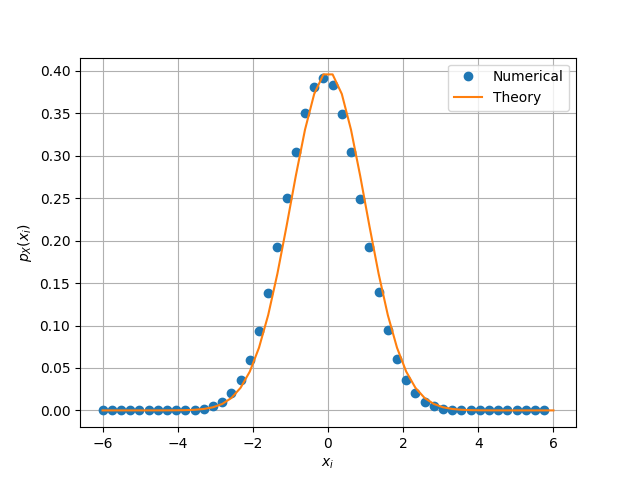
\includegraphics[width=\columnwidth]{figures/pdf.png}
\caption{The PDF of $X$}
\label{fig:gauss_pdf}
\end{figure}
\item Find the mean and variance of $X$ by writing a C program.
\\ \solution \\
Download and execute the following C program
\begin{lstlisting}
wget https://github.com/saanviamrutha/Assignment_rand/blob/main/codes/2.4.c
gcc 2.4.c
./a.out
\end{lstlisting}
Ouput of the program is:
\begin{align}
    mean&=0.000685 \\
    variance&=1.000025 
\end{align}
\item Given that 
\begin{align}
p_{X}(x) = \frac{1}{\sqrt{2\pi}}\exp\brak{-\frac{x^2}{2}}, -\infty < x < \infty,
\end{align}
repeat the above exercise theoretically.\\
%
\solution \\
\begin{align}
    E\sbrak{X} &= \int_{-\infty}^{\infty}x p_{X}\brak{x}~\mathrm{d}x\\
    &=\frac{1}{\sqrt{2\pi}}\int_{-\infty}^{\infty}x\exp\brak{-\frac{x^2}{2}}~\mathrm{d}x\\
    &=0 
\end{align}
$\because x\exp\brak{-\frac{x^2}{2}}$\text{is an odd function.}
\begin{align}
    E\sbrak{X^2} &= \int_{-\infty}^{\infty}x^2 p_{X}\brak{x}~\mathrm{d}x\\
    &=\frac{1}{\sqrt{2\pi}}\int_{-\infty}^{\infty}x^2\exp\brak{-\frac{x^2}{2}}~\mathrm{d}x
\end{align}
Integrating by parts
\begin{multline}
    E\sbrak{X^2} &=\frac{1}{\sqrt{2\pi}}\brak{{x\int x\exp\brak{-\frac{-x^2}{2}}-\int \frac{d\brak{x}}{~\mathrm{d}x}
    &\int x\exp\brak{-\frac{-x^2}{2}}}}
\end{multline}
 \begin{align}
  E\sbrak{X^2} &= \frac{\brak{\brak{-x\exp\brak{-\frac{x^2}{2}}}_{-\infty}^{\infty}+\int_{-\infty}^{\infty}\exp\brak{-\frac{x^2}{2}}}}{\sqrt{2\pi}}\\
   &=\frac{0+\sqrt{2\pi}}{\sqrt{2\pi}}\\
   &=1\\
   var\brak{X}&=E\sbrak{X^2}-\brak{E\sbrak{X}}^2\\
   &=1-0=1
\end{align}
\end{enumerate}
\section{From Uniform to Other}
\begin{enumerate}[label=\thesection.\arabic*
,ref=\thesection.\theenumi]
%
\item
Generate samples of 
%
\begin{equation}
V = -2\ln\brak{1-U}
\end{equation}
%
and plot its CDF. \\
\solution \\
To generate samples of V,download and run the following code.
\begin{lstlisting}
wget https://github.com/saanviamrutha/Assignment_rand/blob/main/codes/v.py
python3 v.py
\end{lstlisting}
The following code plots the CDF of V Fig.\ref{fig:v_cdf} using the samples generated above.
\begin{lstlisting}
wget https://github.com/saanviamrutha/Assignment_rand/blob/main/codes/3_1_cdf.py
python3 3_1_cdf.py
\end{lstlisting}
\begin{figure}
\centering
\includegraphics[width=\columnwidth]{figures/3_1.png}
\caption{The CDF of $V$}
\label{fig:v_cdf}
\end{figure}
\item Find a theoretical expression for $F_V(x)$.
%
\\ \solution \\
The CDF of V is given by
\begin{align}
    F_{V}\brak{x}&=\pr{V\leq x}\\
    &=\pr{-2\ln{\brak{1-U}}\leq x}\\
    &=\pr{1-U\geq \exp\brak{-\frac{x}{2}}}\\
    &=\pr{U\leq 1-\exp\brak{-\frac{x}{2}}}\\
    &=F_{V}\brak{1-\exp\brak{-\frac{x}{2}}}
\end{align}
For \begin{align}
&x\leq 0 & 1-\exp\brak{-\frac{x}{2}}\leq 0 \\
&x>0  & 0<1-\exp\brak{-\frac{x}{2}}<1
\end{align}
\begin{align}
    \implies F_{V}\brak{x}=\begin{cases}
    0  &x\leq 0\\
    1-\exp\brak{-\frac{x}{2}} & x>0
    \end{cases}
\end{align}
\end{enumerate}
\end{document}
